%!TEX root = ../Thesis.tex

\section{Effect of model augmentations and safe mutation}\label{sec: Experimental work: Effects of common model and algorithm augmentations}

\begin{figure}[tbp!]
    \begin{subfigure}[b]{0.49\textwidth}
        \centering
        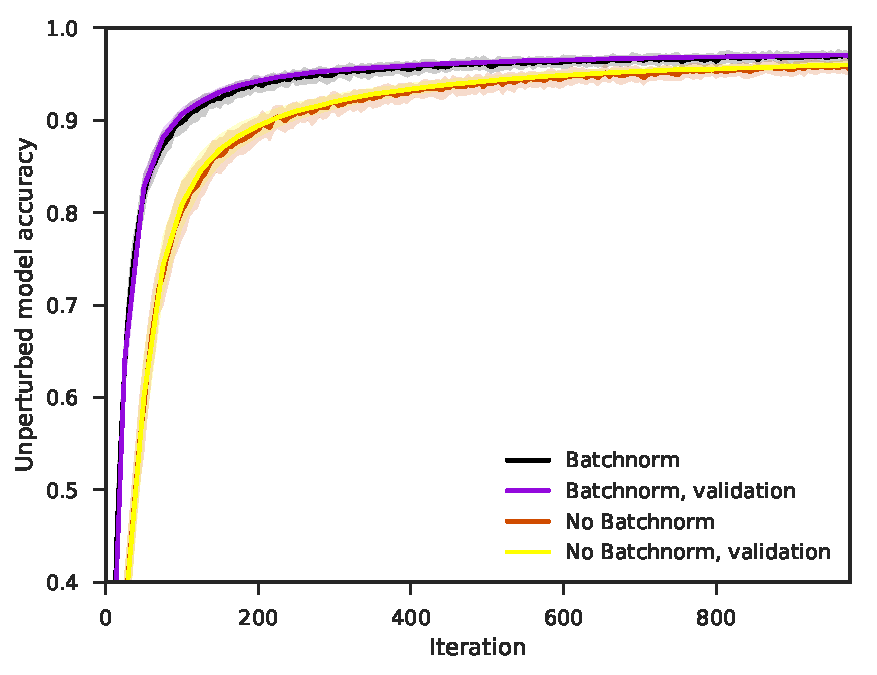
\includegraphics[height=5.8cm]{graphics/E020-bn-analysis/accuracy_unp-all-series-mean-sd.pdf}
        \caption{}
        \label{fig: Theory: E020-bn-analysis/accuracy_unp-all-series-mean-sd}
    \end{subfigure}
    \hfill
    \begin{subfigure}[b]{0.49\textwidth}
        \centering
        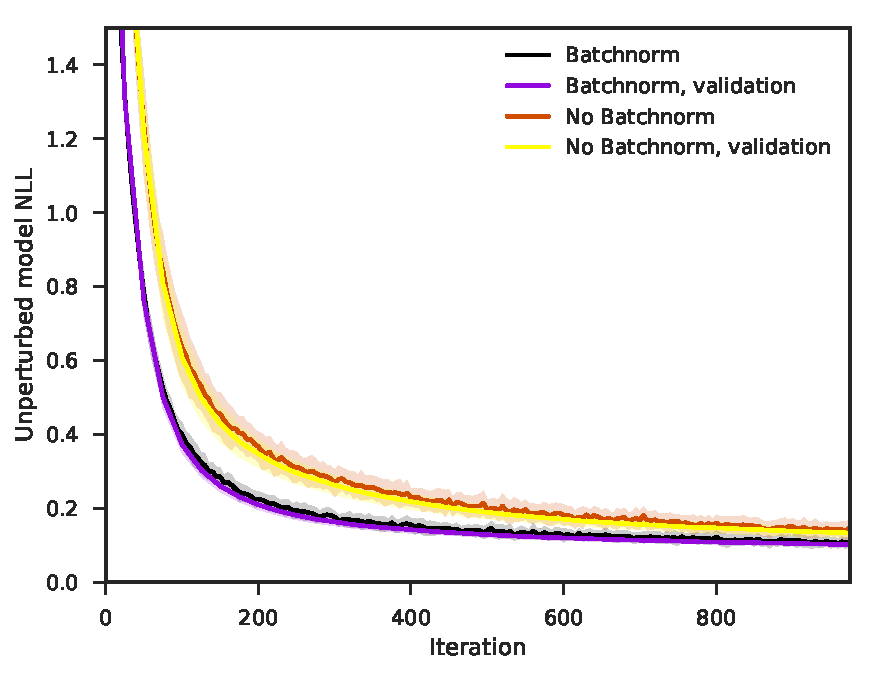
\includegraphics[height=5.8cm]{graphics/E020-bn-analysis/return_unp-all-series-mean-sd.pdf}
        \caption{}
        \label{fig: Theory: E020-bn-analysis/return_unp-all-series-mean-sd}
    \end{subfigure}
    \caption{
        Results of experiments with batch normalization for the unperturbed model.
        \subref{fig: Theory: E020-bn-analysis/accuracy_unp-all-series-mean-sd} Training and validation set classification accuracy.
        \subref{fig: Theory: E020-bn-analysis/return_unp-all-series-mean-sd} Training and validation set \gls{NLL} loss.
        Batch normalization is effective at improving the optimization of the \gls{NN}.
    }
    \label{fig: Theory: E020-bn-analysis}
\end{figure}
This section explores the effects of some common augmentation techniques for \gls{NN} models along with the effects of safe mutation in the \gls{VO} algorithm. The experiments investigate whether the \gls{VO} gradient benefits from the same model improvements as algorithms based on conventional backpropagated gradients do.

The algorithm is isotropic Gaussian \gls{VO} a with fixed variance of $0.05$ similar to \cite{Salimans2017} but uses safe mutation.
%The experiments in this section were performed with the \gls{VO} method listed in \autoref{alg: Canonical variational optimization} using an isotopic Gaussian search distribution but with a fixed $\sigma$ of $0.05$. This algorithm is thus similar to the one used in \cite{Salimans2017} but uses safe mutation.
The experiments were run with 100 perturbations using \gls{SGD} with a momentum of $0.9$ and $L^2$ norm regularization of $0.001$ on all optimized parameters. A learning rate of $0.05$ was used. If nothing else is noted, antithetic sampling and the signed gradient (sum) version of safe mutation were used, batch normalization layers were included in the model and the method of common random numbers was not applied.

The setting is supervised and the data set is \gls{MNIST} for all experiments. The network used is the one for \gls{MNIST} (\autoref{lst: Network models: MNIST with batch normalization}) along with a variant without batch normalization (\autoref{lst: Network models: MNIST without batch normalization}) and a variant without batch normalization and with dropout (\autoref{lst: Network models: MNIST with dropout}).
Each experiment is run for 1000 iterations on mini-batches of 1000 examples for 30 different random seeds. Each experiment shows two plots. The \textbf{(a)} plot shows the classification accuracy for the unperturbed model with each series averaged over the 30 runs at every iteration. The \textbf{(b)} plot shows the \gls{NLL} loss. Both metrics are evaluated on the training set and the test (validation\footnote{The validation set is in fact the remaining part of the data set leaving no data for testing. However, the validation set is not used for fitting any hyperparameters an can as such be regarded a test set as well.}) set during training. The shaded bands indicate one standard deviation among the runs.

Some of these experiments were also run using the Adam optimizer. These plots can be seen in \autoref{app: Effects of common model and algorithm augmentations (Adam optimizer)}. The only difference is the choice of optimizer. The hyperparameter settings for Adam are as recommended in the original paper except for the learning rate which is as for \gls{SGD}. It generally proved to be more difficult to obtain good training characteristics using the Adam optimizer which is hypothesized to be due to the relatively high gradient variance resulting in poor second order moment estimates.


\iffalse
\subsection{Glorot initialization}\label{sec: Experimental work: Glorot initialization}
This section analyzes the results of comparing the default PyTorch initialization scheme with the Glorot initialization scheme \cite{Glorot2010}. \autoref{fig: Theory: E020-init-analysis} shows that initializing the convolutional and linear layers using the Glorot scheme on the \gls{MNIST} network does not yield a signficantly faster learning or better final accuracy compared to the default PyTorch initialization.  In both cases, the learning curves and accuracy curves are almost coincident and within each others standard deviation bands.

That Glorot initialization shows no immediate improvement for the training may here be due to the relatively small network used as well as the simplicity of the problem. Larger networks trained on more challenging data sets may gain more from specialized initialization schemes. Finally, the original paper only applied the scheme to \gls{FNN} without convolutional layers \cite{Glorot2010} which may also influence its effect.

\todo[inline]{WARNING! The default PyTorch initialization is Glorot for linear layers so there really is little difference....}

\begin{figure}[tbp!]
    \begin{subfigure}[b]{0.49\textwidth}
        \centering
        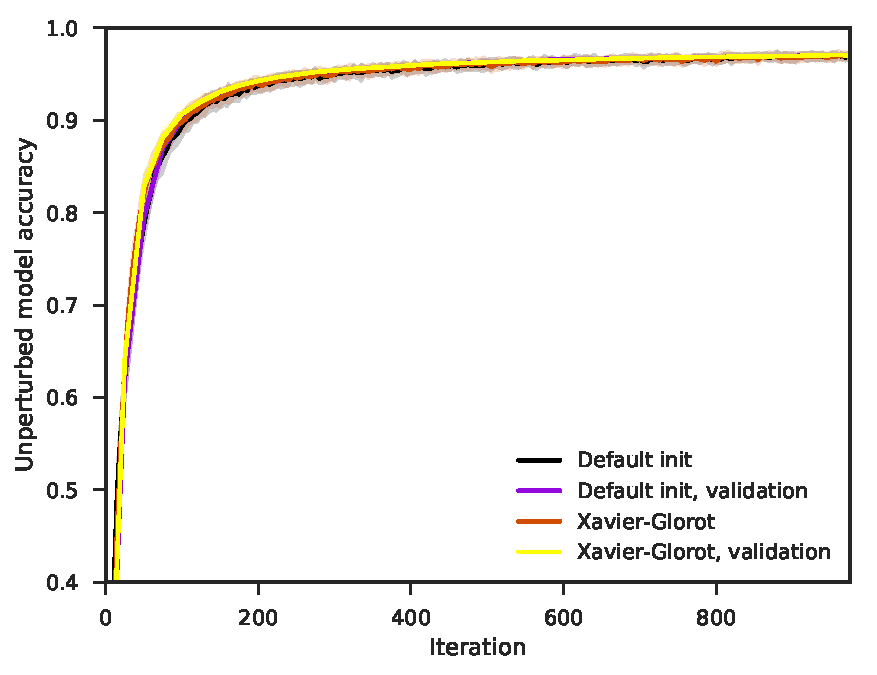
\includegraphics[height=5.8cm]{graphics/E020-init-analysis/accuracy_unp-all-series-mean-sd.pdf}
        \caption{}
        \label{fig: Theory: E020-init-analysis/accuracy_unp-all-series-mean-sd}
    \end{subfigure}
    \hfill
    \begin{subfigure}[b]{0.49\textwidth}
        \centering
        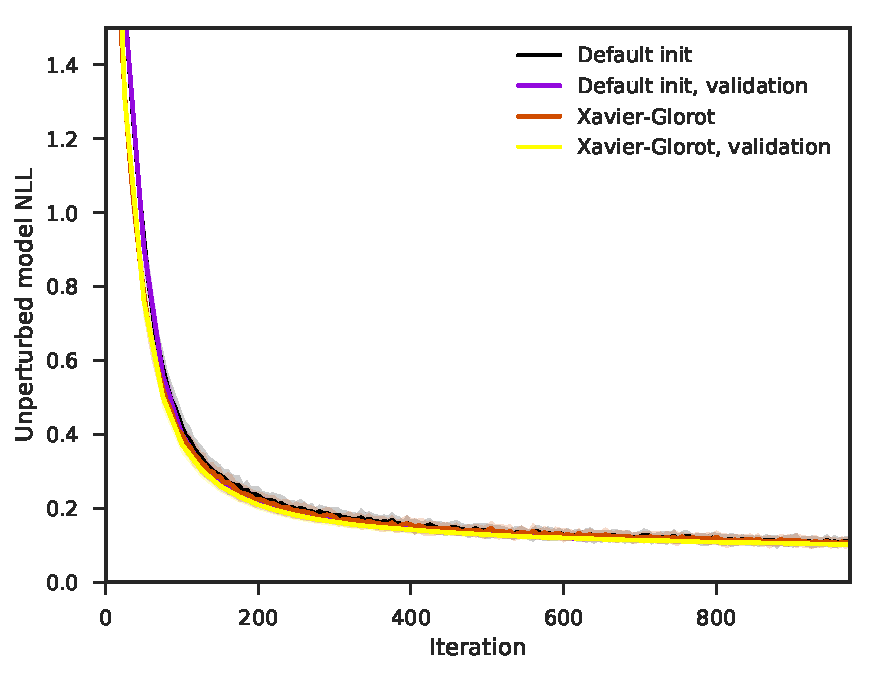
\includegraphics[height=5.8cm]{graphics/E020-init-analysis/return_unp-all-series-mean-sd.pdf}
        \caption{}
        \label{fig: Theory: E020-init-analysis/return_unp-all-series-mean-sd}
    \end{subfigure}
    \caption{
        Results of experiments with initialization scheme for the unperturbed model.
        \subref{fig: Theory: E020-init-analysis/accuracy_unp-all-series-mean-sd} Training and validation set classification accuracy.
        \subref{fig: Theory: E020-init-analysis/return_unp-all-series-mean-sd} Training and validation set \gls{NLL} loss.
    }
    \label{fig: Theory: E020-init-analysis}
\end{figure}
\fi





\subsection{Batch normalization}\label{sec: Experimental work: Batch normalization}
Here, versions of the \gls{MNIST} network with and without batch normalization layers were compared. The positive effect of batch normalization layers between convolution and fully connected layers in the network is evident from \autoref{fig: Theory: E020-bn-analysis}. The network with batch normalization has a significantly steeper loss curve, reaching low losses and high accuracies faster than the network without batch normalization.
It seems the networks asymptote the same final accuracy and loss suggesting that the network without batch normalization is in this case capable of reaching the same level of accuracy as the one with batch normalization, given enough time.
This is in line with the expectated effect of batch normalization as presented in \autoref{chp: Neural networks}. As such, batch normalization can be said to work as expected also with the \gls{VO} gradient which is estimated without the use of backpropagation.



\subsection{Dropout}\label{sec: Experimental work: Dropout}
\begin{figure}[tbp!]
    \begin{subfigure}[b]{0.49\textwidth}
        \centering
        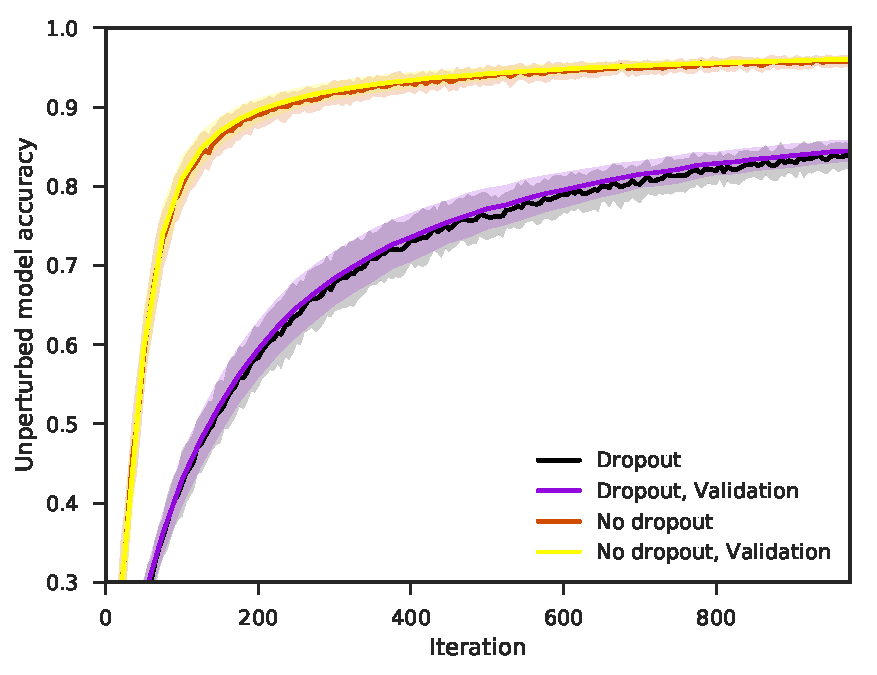
\includegraphics[height=5.8cm]{graphics/E024-DO-SGD-analysis/accuracy_unp-all-series-mean-sd.pdf}
        \caption{}
        \label{fig: Theory: E024-DO-SGD-analysis/accuracy_unp-all-series-mean-sd}
    \end{subfigure}
    \hfill
    \begin{subfigure}[b]{0.49\textwidth}
        \centering
        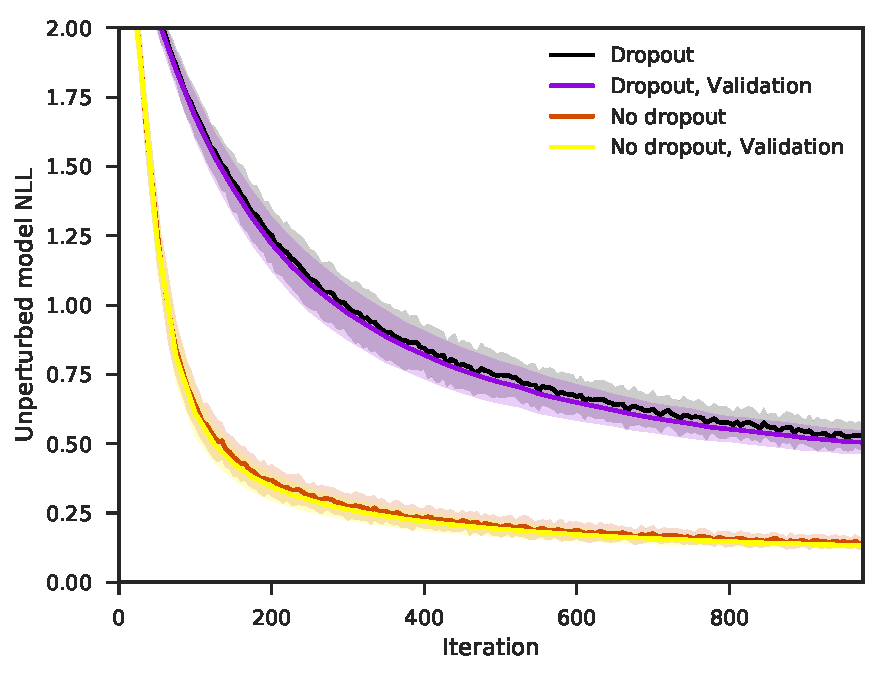
\includegraphics[height=5.8cm]{graphics/E024-DO-SGD-analysis/return_unp-all-series-mean-sd.pdf}
        \caption{}
        \label{fig: Theory: E024-DO-SGD-analysis/return_unp-all-series-mean-sd}
    \end{subfigure}
    \caption{
        Results of experiments with dropout for the unperturbed model.
        \subref{fig: Theory: E024-DO-SGD-analysis/accuracy_unp-all-series-mean-sd} Training and validation set classification accuracy.
        \subref{fig: Theory: E024-DO-SGD-analysis/return_unp-all-series-mean-sd} Training and validation set \gls{NLL} loss. Dropout drastically reduces ease of training probably due to a small network with relatively low capacity and the regularizing effect of optimizing the smoothing \gls{VO} objective.
    }
    \label{fig: Theory: E024-DO-SGD-analysis}
\end{figure}
This section examines the effect of applying dropout to the \gls{MNIST} network. The compared networks are those in \autoref{lst: Network models: MNIST without batch normalization} and \autoref{lst: Network models: MNIST with dropout}, i.e. the network with dropout is compared to a network without dropout. Neither of the networks use batch normalization.

The results of the experiment are shown in \autoref{fig: Theory: E024-DO-SGD-analysis}. The use of dropout results in slower learning and attainment of significantly inferior loss and classification accuracy withing the 1000 iterations. This effect of using dropout is expected to some degree since for the relatively small network used, randomly zeroing weights can drastically reduce model capacity.
Additionally, the \gls{MNIST} network without dropout showed no signs of overfitting in other experiments using the stochastic gradient estimate. As such, dropout was not expected to be able to radically improve performance. 

The fact that no overfitting occurs for this model may be linked to the smoothing of the objective function imposed by using the variational objective. This is most likely a different perspective on the fact that \gls{VO} with a fixed variance optimizes for the average loss of the entire population of perturbations \cite{Lehman2017}. It seems probable that this assists in avoiding overfitting. This observation is also in line with the examples of \autoref{fig: Theory: var-opt-conv-ES-himmelblau}, \ref{fig: Theory: var-opt-conv-VO-R-himmelblau} and \ref{fig: Theory: var-opt-conv-VO-N-himmelblau} where the algorithm with fixed $\sigma$ cannot fully converge on the minimum, and in some sense, thus cannot not overfit it.

\subsection{Safe mutation}
\begin{figure}[tbp!]
    \begin{subfigure}[b]{0.49\textwidth}
        \centering
        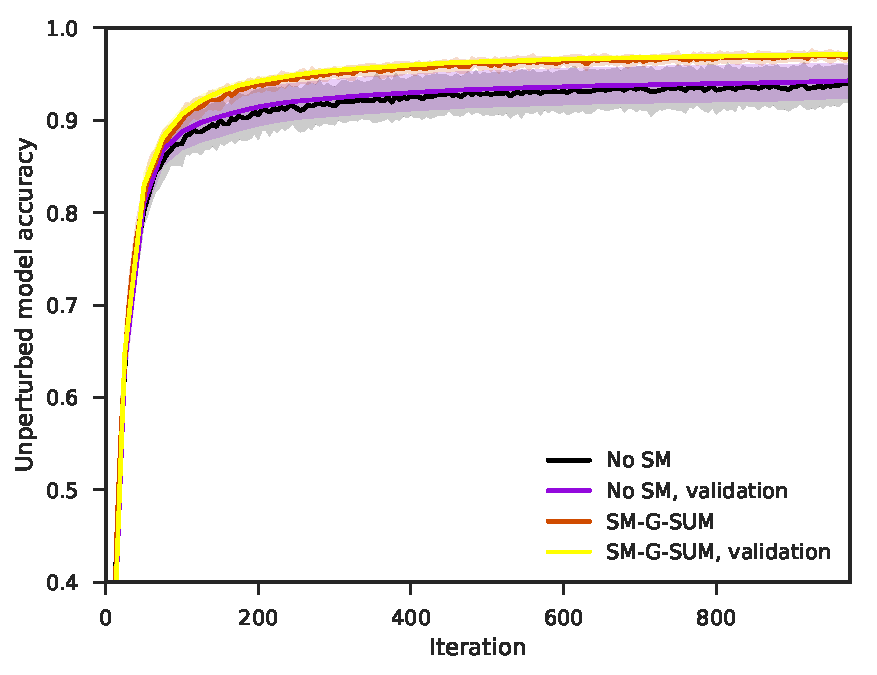
\includegraphics[height=5.8cm]{graphics/E021-SM-analysis/accuracy_unp-all-series-mean-sd.pdf}
        \caption{}
        \label{fig: Theory: E021-SM-analysis/accuracy_unp-all-series-mean-sd}
    \end{subfigure}
    \hfill
    \begin{subfigure}[b]{0.49\textwidth}
        \centering
        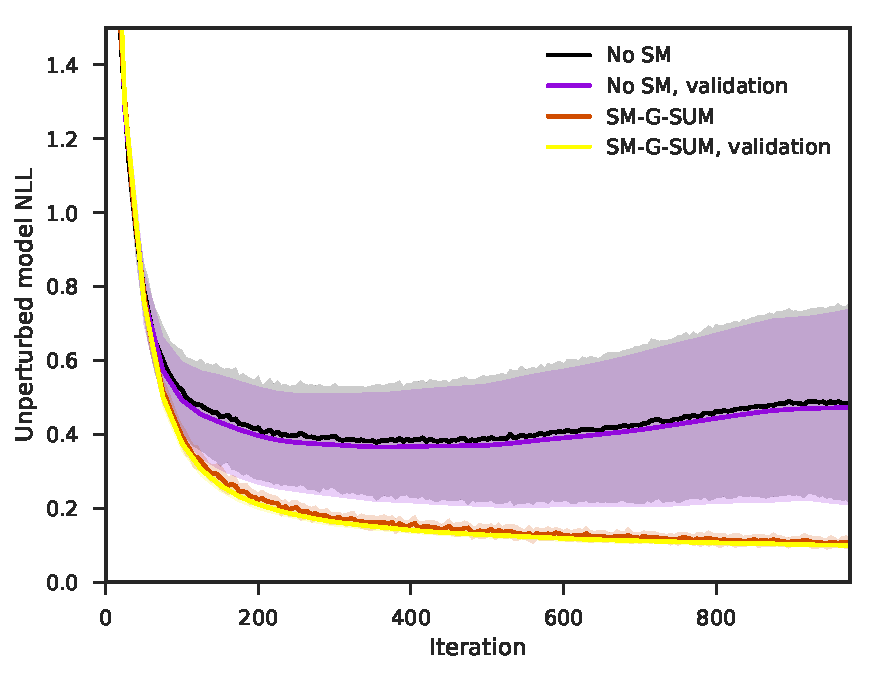
\includegraphics[height=5.8cm]{graphics/E021-SM-analysis/return_unp-all-series-mean-sd.pdf}
        \caption{}
        \label{fig: Theory: E021-SM-analysis/return_unp-all-series-mean-sd}
    \end{subfigure}
    \caption{
        Results of experiments with safe mutation (SM-G-SUM) for the unperturbed model.
        \subref{fig: Theory: E021-SM-analysis/accuracy_unp-all-series-mean-sd} Training and validation set classification accuracy.
        \subref{fig: Theory: E021-SM-analysis/return_unp-all-series-mean-sd} Training and validation set \gls{NLL} loss.
        Scaling perturbations according to network parameter sensitivities results in more stable training.
    }
    \label{fig: Theory: E021-SM-analysis}
\end{figure}
This section compares runs with and without the signed gradient (sum) version of safe mutation \cite{Lehman2017a}.

The results are shown in \autoref{fig: Theory: E021-SM-analysis}. Considering the loss curves, not using safe mutation results in much higher variance among runs with different seeds and yields an over run average loss that is much higher compared to runs using safe mutation. Considering the classification accuracies, the difference between runs with and without safe mutation is smaller although the same trends are observed: Over run variance is higher without safe mutation than it is with and runs without safe mutation reach lower classification accuracies on average. This, along with the high loss, indicates that the variants without safe mutation end up in relatively poor areas of the loss surfaces.

It should be noted that it cannot be ruled out that a lower learning rate exists that allows better performance without safe mutation than what is observed here. For instance, the results presented in \cite{Salimans2017} did not use safe mutation. In this case, the use of safe mutation effectively allows using a higher learning rate which must be expected to result in faster convergence.

\newpage